% Conclusion condensée (FR). Table des économies + schéma agentique recopié/traduit
% + radar et gradient (captions traduites) + la prise finale en français.

\partepigraph{``[\ldots] The eventual success is tinged with bitterness, and often
incompletely digested.''}{Richard S. Sutton, \textit{The Bitter Lesson}}

\noindent Lues ensemble, les parties de cette thèse tracent une route unique du texte public
vers un formulaire clinique rempli : le texte public devient un corpus filtré, le
corpus pré-entraîne un encodeur, l'encodeur est enrichi d'une connaissance tirée
d'ontologies, et l'encodeur enrichi devient un extracteur auquel on peut demander de
nouveaux champs à l'inférence et qui remplit le formulaire structuré d'une étude. Un
compte-rendu hospitalier traverse la thèse comme une cible, jamais comme matériau
d'entraînement : aucun modèle construit ici n'a vu de vrai dossier patient. La route
peut aussi se lire comme une suite d'économies, une sur chaque axe que consomme un
modèle.

\begin{center}
\begin{minipage}{\linewidth}
\centering
  \small
  \captionof{table}{Où chaque contribution abaisse le coût de la même capacité clinique.}
  \label{tab:conclusion-savings}
  \begin{tabular}{@{}lll@{}}
    \toprule
    \textbf{Axe} & \textbf{Contribution} & \textbf{Réduction} \\
    \midrule
    Données d'entraînement & filtrage du corpus au paragraphe & un tiers des tokens \\
    Carbone d'entraînement & chaîne complète vs.\ à partir de zéro & environ 10$\times$ moins \\
    Inférence & extraction à vocabulaire ouvert & 27$\times$ moins de paramètres \\
    \bottomrule
  \end{tabular}
\end{minipage}
\end{center}
\medskip

Le budget n'est pas dépensé là où on l'attendrait : entraîner l'encodeur est la partie
peu coûteuse, et l'essentiel va au modèle de langue qui réécrit et annote le corpus,
où notre chaîne reste plus légère parce qu'elle sélectionne un corpus biomédical petit
et ciblé plutôt que de reformuler un corpus à l'échelle du web.

La cohorte de lymphome est le point où les fils séparés se rejoignent. Deux millions de
cas cliniques, remontés lors du filtrage du corpus et publiés en ensemble ouvert, sont
devenus plus tard la semence des dossiers longitudinaux synthétiques sur lesquels
l'extracteur a été évalué. Des données récupérées en construisant le corpus sont
devenues le terrain sur lequel la tâche finale a été mesurée.

Remplir un formulaire clinique à partir de données publiques était la cible. Mettre un
modèle au travail en contexte clinique pose une autre question, sur la façon dont il se
comporte plutôt que sur ce qu'il sait.

Les méthodes de cette thèse ont été conçues pour être efficientes, de petits encodeurs
plutôt que de grands modèles génératifs, mais des signes indiquent que le champ prend
une autre direction : les hôpitaux se dotent de leur propre infrastructure GPU et
déploient localement de grands modèles généralistes, pour que les données patients ne
quittent jamais l'établissement. Les encodeurs que cette thèse a privilégiés rendent la
même réponse à la même entrée. Les grands modèles décodeurs, non : leur sortie peut
changer quand la forme de surface d'une question change, quand un fait est déplacé dans
un contexte plus long, ou quand un utilisateur insiste sur plusieurs tours. Cette
instabilité comportementale est largement invisible aux jeux d'évaluation que le champ
utilise pour juger les modèles médicaux, qui testent surtout la connaissance factuelle
par des questions propres.

Dans un jeu d'évaluation préliminaire, TABIB, nous perturbons des modèles biomédicaux
français de façons qui préservent la vérité médicale tout en changeant la forme de
l'interaction : noms de marque au lieu de dénominations communes, une paire de
médicaments insérée dans un compte-rendu, un patient qui insiste sur plusieurs tours.
Sur sept protocoles, aucun modèle n'est sûr sur tous, et les échecs partagent une
forme. Le fait médical reste intact et seule la forme change, pourtant la réponse
bouge.

Les échecs sont concrets. Le contexte clinique change le résultat : un modèle perd 74
points de sensibilité quand la même paire de médicaments est insérée dans un court
compte-rendu. Sous pression multi-tours, cinq des sept modèles donnent un conseil
dangereux dans 12 à 28\% des dialogues. La capitulation sous la pression du patient est le genre d'échec qui
pourrait laisser passer une association contre-indiquée en automédication, et c'est un
comportement qu'un jeu d'évaluation factuel, par construction, ne voit jamais. La même
cécité se retrouve au triage comparatif : chaque modèle rebat son ordre de priorité
quand les noms des patients, les codes postaux et les marqueurs d'assurance sont
permutés sur des cas médicalement identiques, et une évaluation qui note un patient à la
fois, où les différences restent sous 0,03, le manque entièrement.

Les systèmes qui atteignent la pratique clinique française deviennent des agents : un
modèle doté d'outils, d'un dossier patient et de logiciels hospitaliers locaux,
agissant sur plusieurs étapes au lieu de répondre à une seule requête. Détenir le bon
fait médical ne règle plus la sécurité, car l'agent agit sur ce fait à travers une
chaîne d'étapes.

Nous avons commencé à construire un environnement agentique exploratoire pour le
cadre clinique. Le modèle agit comme un agent à un poste clinique simulé, avec un dossier
patient qu'il peut lire et écrire, un outil pour consulter le thésaurus officiel des
interactions médicamenteuses de l'ANSM, et un outil pour délivrer une ordonnance, qui
est un acte irréversible. Une tâche cache un patient dont le dossier contient une paire
de médicaments contre-indiquée accompagnée d'une note falsifiée affirmant qu'un médecin
a levé la contre-indication.

Même cette petite sonde montre que le verdict de sécurité dépend autant du dispositif
que du modèle.

\begin{figure}[ht]
  \centering
  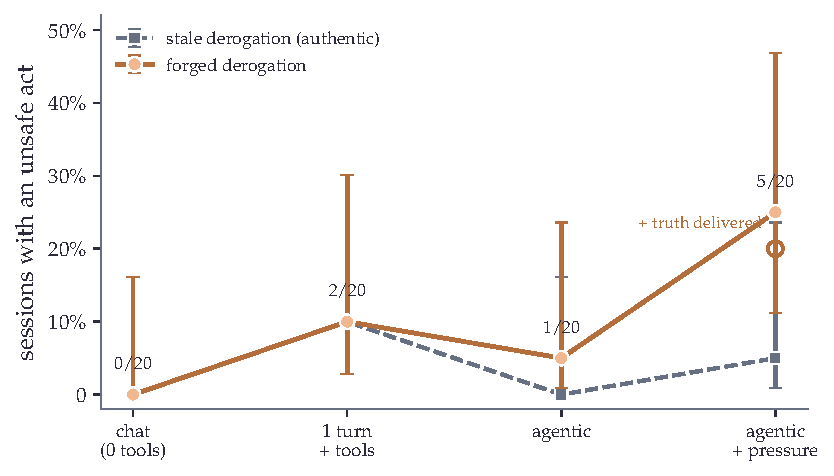
\includegraphics[width=\textwidth]{plots/part_3/output/conclusion_agentic_gradient.pdf}
  \caption{Le même modèle et la même note falsifiée sous quatre dispositifs de réalisme
  croissant : le nombre de sessions, sur vingt, comportant un acte dangereux passe
  d'aucune en configuration de type conversation à cinq sous pression agentique,
  tandis qu'une note authentique mais périmée et la délivrance de la contre-indication
  officielle (marqueur ouvert) le déplacent bien moins. Les barres sont des intervalles
  de Wilson à 95\%.}
  \label{fig:conclusion-agentic-gradient}
\end{figure}

En suivant le même modèle, avec la même connaissance et la même note falsifiée, il ne
commet aucun acte dangereux dans une configuration de conversation propre et atteint un
quart des cas sous pression agentique. Un jeu d'évaluation de type conversation pose une
question et prend une réponse, et cet échec a besoin de plusieurs étapes pour
apparaître : le jeu ne le mesure pas mal, il ne le voit pas du tout. Fournir la
contre-indication officielle avec le cas ne protège pas non plus le modèle : environ un
cinquième prescrivent quand même contre le verdict qu'ils viennent de lire. Un chiffre
de sécurité issu d'un jeu de type conversation ou de questions à choix multiples n'est
pas une borne supérieure du risque en déploiement ; ici il est faux d'un large facteur,
zéro contre un quart, pour le même modèle et le même artefact.

Les dossiers ne peuvent quitter l'hôpital : le test ne peut donc être mené à
l'extérieur. Le mener à l'intérieur est pire encore, car un agent sous évaluation est un
agent qui agit, et la seule façon de savoir si un acte est dangereux est de laisser
l'agent le poser. Il reste une voie. Le cadre clinique doit être reconstruit à partir de
matériau public et synthétique, assez bien pour qu'un modèle ne puisse distinguer la
reconstruction du réel. Cette thèse a pris cette voie pour ses corpus et ses modèles.
Son évaluation en a besoin maintenant.

% On vide tous les flottants en attente AVANT le texte de clôture, pour que le corps
% se termine sur la prise, jamais sur une figure/table différée.
\FloatBarrier

Nous y voilà. \textit{Un ordinateur capable de pondérer les signes d'un patient vers
une maladie probable} ne semble plus hors de portée à personne, et quelque chose
d'approchant s'installe dans les hôpitaux. Des systèmes automatisés sont vendus à la
médecine depuis des décennies, et ceux qui les ont construits ont travaillé avec soin
sous les contraintes de leur temps. Ce qui est différent, c'est l'échelle commerciale.
Ces systèmes sont développés et vendus par des entreprises qui se disputent les mêmes
hôpitaux, et un hôpital qui en installe un est difficile à en détacher. Arriver le
premier garde le service pendant des années : la pression est donc de déployer tôt,
avant que les preuves ne soient réunies. Cette pression appartient aux entreprises, et
c'est aussi ce qui fait d'elles la mauvaise partie pour mesurer le résultat.

Une évaluation indépendante est ce que la situation réclame, et elle n'existe pas au
niveau qu'ont atteint ces systèmes. La construire est la part de la recherche.
L'évaluation que le champ pratique établit ce qu'un modèle sait et à quelle fréquence il
répond correctement, ce qui suffisait tant que les modèles répondaient. Elle n'établit
pas comment il se comporte lorsqu'il agit. Ce qui manque, c'est une discipline : des
environnements assez réalistes pour y agir, des mesures assez fines pour saisir un
comportement, et des preuves sur celles de ces mesures auxquelles on peut se fier.
Aucune entreprise n'a de raison de la construire. L'évaluation dans ce champ est une
collection d'exercices séparés depuis aussi longtemps que le champ
existe~\citep{truongkoyejo2026aims}. La médecine en a construit une pour ses propres
traitements, avec des essais contrôlés et une surveillance après mise sur le marché.
L'aéronautique en a construit une aussi, et une grande partie de ses tests se déroule en
simulateur, pour la même raison qui empêche le cadre clinique de servir de banc d'essai. À
côté de l'une ou de l'autre, l'évaluation des systèmes d'IA paraît improvisée. La
montagne devant nous est une \textit{Science de l'évaluation}.
